\chapter{基于DTW距离度量的Shapelet并行总体方案}
\label{cha:chap03}

本章主要包括基于DTW距离度量的Shapelet并行总体方案和并行化需要解决的问题。并行总体方案部分主要包括Shapelet发现并行框架,并行框架中各个模块的功能,并行框架执行路径的选择。并行化需要解决的问题部分主要是并行设计需要解决的一些关键问题。

\section{基于DTW距离度量的Shapelet并行总体方案}
\label{cha:chap04:myalg:Overview}

Shapelet在实际应用既需要训练模块的离线部分,又需要预测模块的在线部分,因此Shapelet总体方案包括两个部分:离线训练部分和在线预测部分,如图~\ref{fig:kuangjia}。离线训练部分是一个训练模型的过程,输出一个最具有分类能力的子序列。在线预测部分主要是用于对未知的时间序列进行分类和评估预测模型的准确率。
\begin{figure}[H] % use float package if you want it here
	\centering
	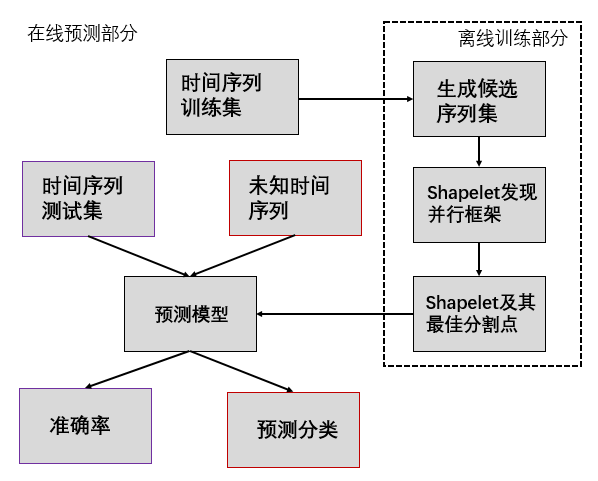
\includegraphics[height=6cm]{kuangjia.png}
	\caption{Shapelet总体方案}
	\label{fig:kuangjia}
\end{figure}

离线训练部分:输入时间序列训练集,根据训练集产生候选序列集,然后在候选序列集上执行Shapelet并行发现过程,将分类能力最高的候选序列及其对应的最佳分割点作为模型输出。模块训练的过程即Shapelet发现的过程非常耗时,模块训练是并行总体方案的重点,本文主要针对这一部分展开叙述的。

在线预测部分:将未知时间序列输入达到预测模型中,预测模型输出其对应的类标。这一部分对于时间消耗非常少,因此不需要进行并行化。

因为离线训练部分Shapelet发现过程非常消耗时间,我们设计了CPU和GPU联合执行的Shapelet发现并行框架,其中CPU负责调度(负责少量数据计算),GPU负责执行数据计算,章节~\ref{cha:chap04:myalg:Overview:overallScheme}主要介绍发现过程的整体框架。发现过程方案中的多个模块对于Shapelet发现过程的三阶段功能进行了实现,章节~\ref{cha:chap03:modelduty}主要介绍各个模块的功能。因为数据集和距离参数的不同,Shapelet发现过程在同一阶段的执行中会选择不同的模块,章节~\ref{cha:chap03:parachoose}介绍了数据流向如何根据数据集和距离参数进行选择。

\subsection{Shapelet发现并行框架}
\label{cha:chap04:myalg:Overview:overallScheme}

\begin{figure}[H] % use float package if you want it here
	\centering
	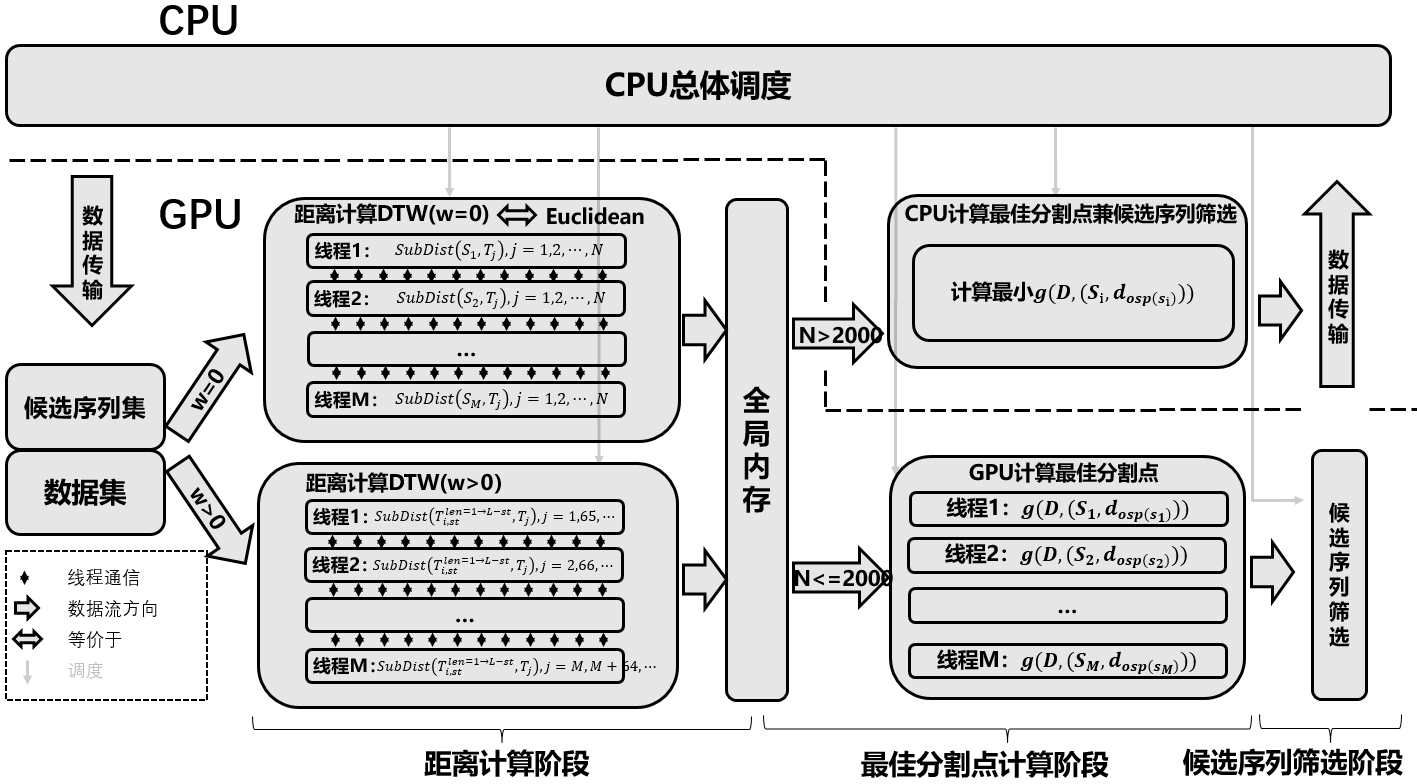
\includegraphics[height=8.3cm]{generalflowchart.png}
	\caption{Shapelet发现并行框架}
	\label{fig:generalflow}
\end{figure}

图~\ref{fig:generalflow}基于DTW距离度量的Shapelet并行算法发现过程的并行框架图。输入数据是数据集和候选序列集,其中候选序列集是对于时间序列的所有子序列枚举获得。输出数据是一个具有高分类能力的候选序列及其最佳分割点等作为预测模型。框架部分包括六个模块:w>0距离计算模块、w=0距离计算模块、GPU最佳分割点计算模块、CPU最佳分割点计算模块、候选序列筛选模块、全局内存(中间变量存储),这六个模块分别对于Shapelet发现过程的三阶段进行实现,各模块的功能会在章节~\ref{cha:chap03:modelduty}介绍。三个阶段的功能如下:

1.距离计算阶段:输入候选序列集$S$和数据集$D$,输出多个$\mathcal{F}$并且存储在全局内存中(见定义~\ref{def:chap2:SubDist},公式~\ref{equ:chap2:SubDistSet}),其中包括w>0距离计算模块和w=0距离计算模块。 

2.最佳分割点计算阶段:输入多个$\mathcal{F}$(从全局内存读入),输出信息增益$g(D,(S,d_{osp(S)}))$以及对应的$S$,$d_{osp(S)}$,包括CPU最佳分割点计算模块和GPU最佳分割点计算模块。

3.候选序列筛选阶段:输入多个候选序列$S$以及对应的信息增益$g(D,(S,d_{osp(S)}))$,最佳分割点$d_{osp(S)}$,输出具有最大信息增益的$S$以及对应的$d_{osp(S)}$,实现模块为候选序列筛选模块。

Shapelet发现过程根据不同的数据集和不同的扭曲匹配程度选择不同的执行模块,如何进行执行路径的选择会在章节~\ref{cha:chap03:parachoose}介绍。

\subsection{并行框架各模块功能}
\label{cha:chap03:modelduty}

本章节主要介绍并行框架中的六个模块:w>0距离计算、w=0距离计算、GPU最佳分割点计算、CPU最佳分割点计算、候选序列筛选、中间变量存储(全局内存)。

\textbf{中间变量存储模块(全局内存)}:全局内存承担距离计算阶段和最佳分割点计算阶段的中间媒介,距离计算阶段将距离计算结果$\mathcal{F}$存入全局内存,最佳分割点计算阶段再从全局内存读取$\mathcal{F}$来计算最佳分割点,其中距离计算阶段和最佳分割点计算阶段都使用合并内存访问Coalesced的方法,从而减少全局内存访存延时。

\textbf{w>0距离计算模块}:距离度量采用$DTW(A,B,w)$,每个线程主要负责$T_i$中以$s$位置为起始的所有候选序列$\left\lbrace T_{i,s}^{len},len=1\to L-s\right\rbrace $和数据集$D$中几个时间序列$T_j$的距离计算,然后将其存入全局内存相应位置,如公式~\ref{equ:chap04:everythread2},具体实现细节会在章节~\ref{cha:chap04:myalg:DTW}介绍。
%\begin{equation}
%\label{equ:chap04:everythread2}
%\begin{array}{l}
%SubDist(T_{i,s}^{len},T_j), \\ [0.3cm]
%s.t.~ len=1\to(L-s),j=\left\lbrace tid_x,tid_x+dim_{tidx},tid+2*dim_{tidx},\cdots \right\rbrace  
%\end{array}
%\end{equation}
\begin{equation}\label{equ:chap04:everythread2}
\left\{\begin{array}{l}
\left\lbrace SubDist(T_{i,s}^{len},T_j) \right\rbrace \\[0.1cm]
\mbox{subject to:}\\[0.1cm]
\qquad len=1\to (L-s)\\[0.1cm]
\qquad j=\left\lbrace tid_x,tid_x+dim_{tidx},tid+2*dim_{tidx}\right\rbrace 
\end{array}\right.
\end{equation}

\textbf{w=0距离计算模块}:距离度量采用$Euclid(A,B)$,每个线程执行一个候选序列$S$相对于数据集$D$所有时间序列$T_j$计算距离$\mathcal{F}=SubDist(S,T_j),j=1\to N$,最后将$\mathcal{F}$存入全局内存相应位置。某个线程块Block负责一个时间序列的长度为$len$的子序列,比如线程块$Block(i,len)$计算候选序列就是$T_{i,s}^{len},s=1,2,\cdots,L-len+1$。$w=0$距离计算模块算法中线程存在依赖关系,需要线程之间进行协作计算,详见章节~\ref{cha:chap04:myalg:euclid}。相比于w>0距离计算模块,本模块减少不必要的访存过程和比较过程。当然算法也是有缺陷的,时间序列长度$L$不能超过1024,因为线程之间需要通信才能完成依赖计算,GTX 1080一个线程块Block中最多允许1024个线程,超过1024个线程的依赖关系不能建立。

\textbf{GPU最佳分割点计算模块}:从全局内存读取$\mathcal{F}$,然后并行计算候选序列对应的最佳分割点$d_{osp}$,这里使用了启发式算法计算最佳分割点,详细设计见章节~\ref{cha:chap04:myalg:infogain}。本模块会根据不同$N$大小使用不同的共享内存及寄存器改变相应的$grid$和$block$参数,使尽可能多的线程同时并行计算。

\textbf{CPU最佳分割点计算模块}:采用的算法和GPU最佳分割点计算模块的算法是相同的,不同的是在CPU中执行。当N增大到一定程度时,流处理器簇SM上的资源不再足够32个线程执行,就会切换到CPU执行。

\textbf{候选序列筛选模块}:最佳分割点阶段产生$O(NL^2)$个候选序列$S$及其对应的信息增益$g(D,(S,d_{osp(S)}))$和分割点$d_{dsp(S)}$,在本模块中需要选出具有最大信息增益的候选序列及其对应的分割点。本模块的本质是一个特大向量求最大值的过程,是一个典型的归约过程,可以采用并行归约的算法求最大信息增益,时间复杂度为$O(\log(N)+\log(L))$。我们这里并没有直接使用归约算法,而是将原始归约算法~\cite{harris2007optimizing}的求最大值过程改造成求最大值索引过程,这样能够避免候选序列和分割点跟随信息增益一起归约。因为并行求最大信息增益过程总的时间占比不超过1\%,本文不做过多的介绍。另外,正因为候选序列筛选模块是一个归约过程,为了保持高效率,使用独立的并行计算完成。

\subsection{并行框架执行路径的选择}
\label{cha:chap03:parachoose}

$w$的取值是控制扭曲匹配程度的参数,当$w>0$时,距离计算阶段采用的距离度量是$DTW(A,B,w)$;而当$w=0$时,为了避免不必要的计算,距离计算阶段采用$DTW(A,B,w)$距离度量的等价方案$Euclid(A,B)$。因此,距离计算阶段会根据$w$的不同分为不同的模块:w>0距离计算模块和w=0距离计算模块。另外,一个线程块Block中最多出现1024个线程,$w=0$距离计算模块允许最长的时间序列长度$L$为1024(线程之间需要协作)。

因此,当$w>0$或$L>1024$时,执行w>0距离计算模块;而当$w=0$且$L<=1024$时,执行w=0距离计算模块。

GPU上多线程计算最佳分割点,每个线程需要$O(N)$的空间,但是硬件环境每个线程块Block只能提供48K的共享内存和64K的寄存器大小(见表~\ref{tab:gpuversion}),可能会出现内存不足或者过大内存需求导致每个流处理器簇SM上运行的线程束Warp个数减小。虽然通过调节线程块Block的参数能够一定程度上缓解这种情况,但是依然存在这样一个阈值,当$N$大于这个阈值时,GPU将不能提供足够的资源进行最佳分割点并行计算。

因此,设定一个阈值$N_{th}=2000$(根据一个$block$执行32个线程所需资源计算),当$N\leq N_{th}$时,最佳分割点计算时,执行GPU最佳分割点计算模块;当$N>N_{th}$时,执行CPU最佳分割点计算模块,其中CPU最佳分割点模块的算法和GPU最佳分割点模块相同。

对于w>0距离计算模块、w=0距离计算模块、最佳分割点计算模块,会估计不同数据集即不同$w,N,L$参数下每个线程块Block中共享内存和寄存器的使用情况。本文对于不同的$w,N,L$设置了资源使用上线,会根据不同的参数调节线程块Block和计算网格Grid参数,避免单个Warp占用资源太多,而影响流处理器SM上同时执行的线程束Warp个数,这样可以使有限的资源上进行更多的计算。


\section{并行化需要解决的问题}

本章节主要介绍设计并行化之前需要解决的问题,包括中间变量$\mathcal{F}$的存储问题、特定需求的矩阵转置问题、最佳分割点计算的时间复杂度问题。

\subsection{中间变量$\mathcal{F}$的存储问题}
\label{cha:chap03:Problemsencountered:BigDataSet}

$\mathcal{F}$是计算Shapelet中计算距离阶段和最佳分割点阶段的中间变量,空间复杂度为$O(N)$,对于整个候选序列集而言,$\mathcal{F}$存储的空间复杂度为$O(N^2L^2)$,所需要的空间大小取决于数据集的大小,根据不同的数据集大小,有不同的方案,具体如下:

当数据集大小及时间序列长度$N,L$很小的时候,我们采用寄存器存储$\mathcal{F}$,不会涉及到访存延时,计算速度会很快。

当$N,L$增大时,寄存器不见不能满足存储要求,系统会逐渐使用局部内存(局部内存实际上占用全局内存,和全局存储速度一致,但是又没有使用合并内存访问,会有很大的访存延时),因此各线程会出现频繁的访存延时而使性能非常差。因为有限的寄存器和共享内存都不能满足$\mathcal{F}$存放的要求,这里我们考虑将$\mathcal{F}$放在全局内存中存储。使用全局内存保证$\mathcal{F}$的存储空间,为了保证执行效率,距离计算阶段必须通过合并内存访问Coalesced的方法将$\mathcal{F}$存储到全局内存,最佳分割点计算阶段必须通过合并内存访问Coalesced的方法从全局内存读取$\mathcal{F}$。

将$\mathcal{F}$放在全局内存中存储,只能一定程度上解决资源不足的问题。当$N,L$继续增大时,全局内存依旧不能满足$\mathcal{F}$的资源需求,全局内存肯定不能提供平方级别的空间需求,$O(N^2L^2)$的空间复杂度会使$\mathcal{F}$需要的内存很快超过全局内存大小。对于全局内存不能中间结果$\mathcal{F}$空间不足的情况,这里使用换入换出~\cite{li2016data}的思路去解决,将整个候选序列集分为多个子集,每次对于一个候选序列子集在GPU中进行Shapelet并行发现过程,再在CPU上综合多次计算的结果,同时使用合并内存访问和延时隐藏保证效率,具体如图~\ref{fig:Swapinout}。当然有多块GPU可供使用时,也可以多个GPU同时并行多个候选序列子集,然后再统一归约。这里涉及的换入换出、数据在主机和GPU之间拷贝,不再这里详述。

\begin{figure}[H] % use float package if you want it here
	\centering
	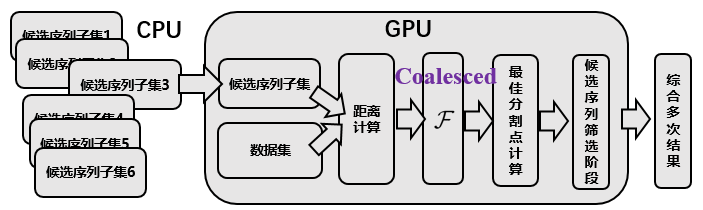
\includegraphics[width=12.2cm]{Swapinout.png}
	\caption{中间变量$\mathcal{F}$存储空间需求过大的解决方案}
	\label{fig:Swapinout}
\end{figure}

这里解释一下为什么从$\mathcal{F}$中间变量处分为距离计算和最佳分割点计算两个阶段,主要三个原因:

1.距离计算阶段和最佳分割点计算阶段是不同性质的计算,将两者分开更有利于保持各线程均衡,有利于资源的充分利用;

2.在距离计算阶段,后文根据$w$的不同分为$w>0$距离计算模块和$w=0$距离计算模块,两者访问$\mathcal{F}$的方式不同;

3.从$\mathcal{F}$处分开有利于算法实现,使每个$kernel$的功能都比较清晰。


\subsection{特定需求的矩阵转置}

在$w=0$距离计算模块中,每个线程块Block都会产生一个矩阵,我们需要将每一个矩阵中的列向量变成行向量,这时候就需要采用矩阵转置过程。但是这里我们不能使用CUBLAS~\cite{chrzeszczyk2013matrix}中库或者或现成算法,原因有两点:

第一:如图~\ref{fig:customtranspose},每一个线程块Block产生一个$M*N$的矩阵都存储在全局内存一个$C*R$的一个块中,矩阵并没有占据整个块的空间;每个线程块Block产生矩阵列数$M$不一致,但是$C,R$的大小是根据最大的$M,N$确定,而$M$的差别有可能很大,如图~\ref{fig:customtranspose}中的$Block_1$和$Block_2$。调用算法的矩阵转置都是按照$C*R$的大小进行转置的,有可能造成大量计算资源浪费。

第二:我们这里要求转置之后的矩阵行与行之间是拼接起来的,如图~\ref{fig:customtranspose}右侧部分。如果调用现成算法的矩阵转置之后的每个矩阵之间都会出现空白,如果需要按行拼接起来,必须再进行一次全局内存拷贝过程,这样同样违背我们加速的目的。

我们需要设计一个矩阵转置算法能够做到资源合理利用,可以从以下两个角度进行:

1.对于不同大小的矩阵,根据矩阵的实际大小进行转置,转置的大小不能$(M+32,N+32)$;

2.计算每个矩阵转置拼接之后的偏移和行数,方便直接转置到偏移位置。
\begin{figure}[H] % use float package if you want it here
	\centering
	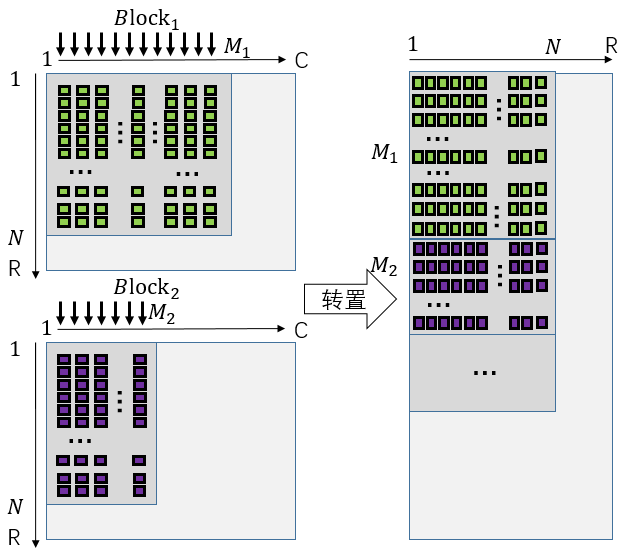
\includegraphics[height=9cm]{customtranspose.png}
	\caption{特定矩阵转置要求}
	\label{fig:customtranspose}
\end{figure}
\subsection{最佳分割点计算的时间复杂度问题}

距离计算阶段的时间复杂度为$O(N^2L^4)$,距离计算是Shapelet发现复杂度最高的计算。但是距离计算阶段的时间复杂度可以降到$O(N^2L^3)$,最佳分割点计算阶段的时间复杂度为$O(N^2L^2\log(N))$。

当数据集$D$很大时,即$N$很大时,最佳分割点阶段有可能成为Shapelet发现过程占比时间最大的计算。我们需要降低最佳分割点计算的时间复杂度,从而降低执行时间。

传统的最佳分割点计算,对于所有可能的阈值$d_{th}$都进行了尝试,如~\ref{equ:chap3:Infogain}。一般会将$\mathcal{F}$按照距离进行排序(排序时间复杂度$O(N\log(N))$)之后,以每两个距离之间的值作为阈值$d_{th}$进行尝试,这是以一种遍历的方法寻找全局最优值。
\begin{equation}
\label{equ:chap3:Infogain}
	g(D,(S,d_{osp(S)})) \geq g(D,(S,d_{th})),\forall d_{th}\in \mathbb{R}_{+}
\end{equation}

但是我们的目的不是对于距离进行排序,我们是需要找一个阈值$d_{th}$,将数据集$D$中的两类尽可能分开。这里可以采用一种启发式的搜索方法,搜索满足条件的阈值。因为候选序列非常多,可以使用不同的搜索方式来使其中一种候选序列产生的阈值尽量靠近全局最优值,具体的方案将在章节~\ref{cha:chap04:myalg:infogain}中介绍。

\section{本章小结}

本章首先从应用角度介绍了基于DTW距离度量的并行Shapelet的并行总体方案,包括在线预测部分和离线训练部分。因为离线训练部分比较耗时,我们提出了Shapelet发现的并行框架,并对于框架内的各个模块功能和如何在模块之间进行数据流向的选择进行了介绍。然后本章还对于并行化之前需要解决的问题进行了详细叙述。



